\section{Language-driven Semantic Segmentation}
\label{sec:method}
\begin{figure}[t]
    \centering
     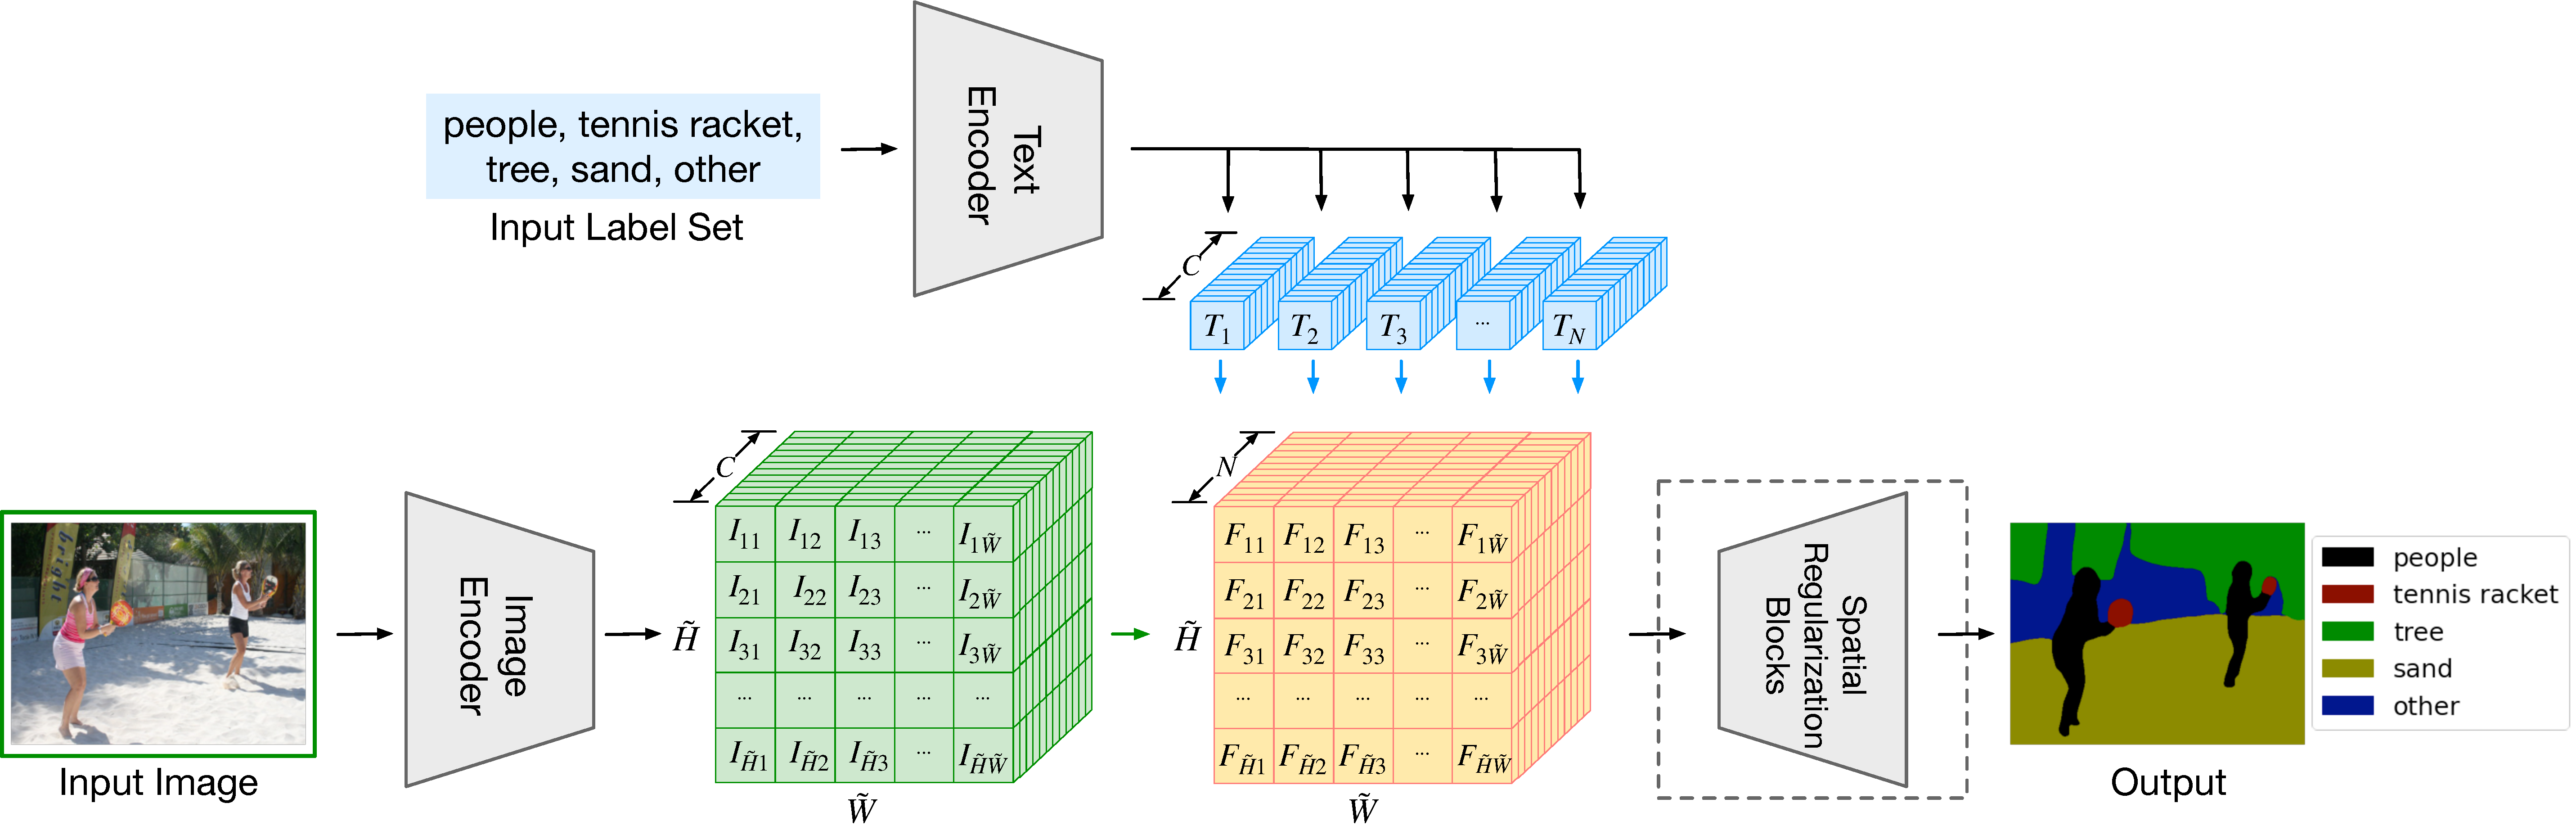
\includegraphics[width=\linewidth]{imgs/main_arch.pdf}
    \caption{Overview. A text encoder embeds labels into a vector space. An image encoder extracts per-pixel embeddings from the image and correlates the feature of each pixel to all label embeddings. The image encoder is trained to maximize the correlation between the text embedding and the image pixel embedding of the ground-truth class of the pixel. A final spatial regularization block spatially regularizes and cleans up the predictions.  
    }
    \label{fig:main_arch}
    \vspace{-0.1in}
\end{figure}


Our approach, \emph{Language driven Semantic segmentation (\methodname{})} embeds text labels and image pixels into a common space, and assigns the closest label to each pixel. We illustrate the framework in Figure~\ref{fig:main_arch} and describe each part in detail below. 

\paragraph{Text encoder.}
The text encoder embeds the set of $N$ potential labels into a continuous vector space $\mathbb{R}^C$, producing $N$ vectors $T_1,\dots,T_n\in{\mathbb{R}^C}$ as outputs (blue vectors in Figure~\ref{fig:main_arch}). Multiple network architectures are possible, and we use the pretrained Contrastive Language–Image Pre-training (CLIP) throughout~\citep{radford2021learning}. 
By design, the set of output vectors is invariant to the ordering of the input labels and allows their number, $N$, to vary freely. 


\paragraph{Image encoder.} Similar to the text encoder, the image encoder produces an embedding vector for every input pixel (after downsampling). 
We leverage dense prediction transformers (DPT)~\citep{ranftl2021vision} as the underlying architecture. Assume $H\times W$ is the input image size and $s$ is a user-defined downsampling factor ($s=2$ in our implementation). We define $\tilde{H} = \frac{H}{s}$, $\tilde{W} = \frac{W}{s}$. The output is a dense embedding    $I\in{\mathbb{R}}^{\tilde{H}\times\tilde{W}\times C}$ (green tensor in Figure~\ref{fig:main_arch}). We refer to the embedding of pixel $(i,j)$ as $I_{ij}$. 

\paragraph{Word-pixel correlation tensor.} After the image and the labels are embedded, we correlate them by the inner product, creating a tensor of size $\tilde{H}\times\tilde{W}\times N$ (orange tensor in Figure~\ref{fig:main_arch}), defined as
\begin{align}
    f_{ijk} = I_{ij} \cdot T_{k}. 
\end{align}
We refer to the $N$-dimensional vector of inner products between the embedding of pixel $(i,j)$ and all $N$ words as $F_{ij} \in \mathbb{R}^N$, where $F_{ij} =  (f_{ij1}, f_{ij2}, ..., f_{ijk})^T$.
During training, we encourage the image encoder to provide pixel embeddings that are close to the text embedding of the corresponding ground-truth class. Specifically, given the text embeddings $T_k \in \mathbb{R}^C$ of $N$ labels and the  image embedding $I_{ij} \in \mathbb{R}^C$ of pixel $i,j$, we aim to maximize the dot product of the entry $f_{ijk}$ that corresponds to the ground-truth label $k=y_{ij}$ of pixel $i,j$. We achieve this by defining a pixelwise softmax objective over the whole image:
 \begin{align}
      \sum_{i,j=1}^{H, W} \textrm{softmax}_{y_{ij}}\left(\frac{ F_{ij}}{t}\right),
 \end{align}
where $t$ is a user-defined temperature parameter that we set to $t=0.07$~\citep{wu2018unsupervised,radford2021learning}. During training, we minimize a per-pixel softmax with cross-entropy loss (with temperature scaling) as is standard in semantic segmentation\footnote{In practice we implement this using the standard nn.CrossEntropyLoss from Pytorch.}.





\begin{wrapfigure}{R}{0.4\linewidth}
    \centering
     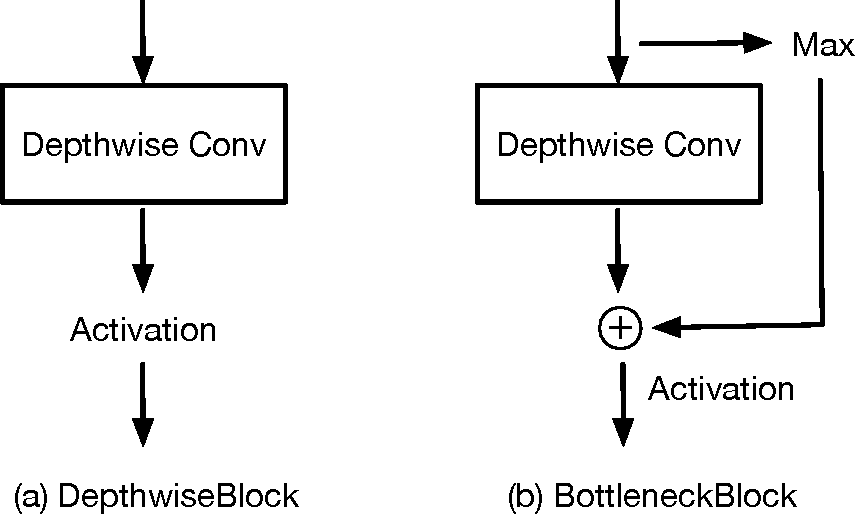
\includegraphics[width=0.9\linewidth]{imgs/main_blocks.pdf}
    \caption{Illustration of \bottleneckblock{} and \depthwiseblock{}.}
    \label{fig:main_blocks}
    \vspace{-0.1in}
\end{wrapfigure}
\paragraph{Spatial regularization.}
Due to memory constraints, the image encoder predicts pixel embeddings at lower resolution than the input image resolution. We use
an additional post-processing module that spatially regularizes and upsamples the predictions to the original input resolution. 
During this process, we have to ensure that all operations stay equivariant with respect to the labels. In other words, there should be no interactions between the input channels, whose order is defined by the order of the words and can thus be arbitrary. We evaluate two functions that fulfill this property: a simple cascade of depthwise convolutions~\citep{chollet2017xception} followed by non-linear activations (DepthwiseBlock), and another block that additionally augments the depthwise convolutions with the result of a max-pooling operation over the set of labels (BottleneckBlock)~\citep{li2019positional}. In a final step we use bilinear interpolation to recover predictions at the original resolution. We refer to these functions as ``spatial regularization blocks'' and illustrate them in Figure~\ref{fig:main_blocks}.



\paragraph{Training details.}
We initialize the backbone of the image encoder with the official ImageNet pretrained weights from ViT~\citep{dosovitskiy2020image} or ResNet~\citep{he2016deep}\footnote{We also evaluated on a model initialized with the CLIP image encoder with the same setup and hyperparameters, but observed worse performance than using the ViT initialization.} and initialize the decoder of DPT randomly. During training we freeze the text encoder and only update the weights of the image encoder. We provide the full label set that is defined by each training set to the text encoder for each image. 


Our model can be trained on any semantic segmentation dataset and supports flexible mixing of multiple datasets through the text encoder.
Existing semantic segmentation models assign a fixed channel in the output to represent the probability of a pixel being the corresponding semantic class. In contrast, our approach can dynamically handle label sets with varying length, content, and order. This property
allows synthesizing arbitrary zero-shot semantic segmentation models by simply changing the labels that are fed to the text encoder. 

